\documentclass{article} % this tells LaTeX to make an article (as opposed to a book, for example)

\usepackage[utf8]{inputenc}
\usepackage[english]{babel}
\usepackage{indentfirst}


\usepackage{amsmath, % this adds functions for formatting equations nicely
      amssymb,
      multirow,
      multicol,
      amsthm,
      todonotes, % add to do notes with \todo command
      mathtools,
      stmaryrd,
      tikz } % this gives us lots of greek symbols
\usepackage{titling}
\usepackage{pgfplots}
\usepackage[round]{natbib} % extra functionality for citations
\usepackage{tikzscale}
\usetikzlibrary{backgrounds}

\usetikzlibrary{arrows.meta,positioning,calc,automata, arrows}
\pgfplotsset{compat=1.16}

\newcommand*\circled[1]{\tikz[baseline=(char.base)]{
            \node[shape=circle,draw,inner sep=2pt] (char) {#1};}}
\newcommand*\circleditem{%
   \stepcounter{enumi}\item[\circled{\theenumi}]}


\setlength{\parskip}{1em}

\newtheorem{theorem}{Theorem} 
\newtheorem{definition}{Definition} % this lets us create definition blocks as below
\newtheorem{remark}{Remark}
\newtheorem{lemma}[theorem]{Lemma}

\usepackage{thmtools}
\usepackage{thm-restate}

\usepackage{hyperref}

\usepackage{cleveref}

\declaretheorem[name=Theorem]{thm}

\title{A Graph Theoretical Approach to Revealed Preferences and Efficiency Indices}
\author{...}
\begin{document}

\maketitle

\begin{abstract}
Prior literature on consumer behavior and revealed preferences focus on the necessary requirements of choice data to satisfy consistency but often neglect developing algorithms to test for those requirements and calculate existing efficiency indices on large datasets. This paper places existing theory in a graph theoretical context and discusses canonical algorithms to test for consistency. Additionally, this paper offers an alternative algorithm to directly calculate efficiency indices proposed by \citet{Afriat1967The-Construction-of-Utility-Functions-from-Expenditure-Data} and \citet{Varian1990Goodness-of-fit-in-optimizing-models} through the application of tropical semiring on adjacency matrices.
\end{abstract}

\section*{Existing Literature and Axioms}

Suppose an individual is observed over $k$ (a finite number of) periods. Let $\mathcal{X}=\{X_1,\ldots,X_k\}$ be the set of quantity vectors such that $\forall i\in\{1,\ldots,k\}$, $X_i=(x_{i1},\ldots,x_{in})$, where $x_{ij}$ represents the number of good $j$ bought at time $i$. Further, let $\mathcal{P}=\{P_1,\ldots,P_k\}$ be the set of price vectors constructed in similar fashion as the quantity vectors. We then define a following set of relations between elements of $\mathcal{X}$:

\begin{definition}\label{defn:relations_1} \leavevmode
\begin{enumerate}
  \circleditem For $X_i, X_j\in\mathcal{X}$, we say $X_i$ is \textbf{directly revealed preferred} to $X_j$ if $P_iX_i\geq P_iX_j$. We will denote this as $X_i R_D X_j$.
  \circleditem For $X_i, X_j\in\mathcal{X}$, we say $X_i$ is \textbf{strictly directly revealed preferred} to $X_j$ if $P_iX_i>P_iX_j$. We will denote this as $X_i R_{SD} X_j$.
  \circleditem For $X_i, X_j\in\mathcal{X}$, we say $X_i$ is \textbf{revealed preferred} to $X_j$ if there exists some sequence $\{X^m\}_{m=1}^{M}$ such that, $\forall m\in\{1,\ldots,M\}$, the following holds:
  \begin{itemize} 
    \item $X^m\in\mathcal{X}$
    \item $X_i R_D X^1$
    \item $X^m R_D X^{m+1}$
    \item $X^M R_D X_j$
  \end{itemize} 
  We will denote this as $X_i R X_j$.
\end{enumerate}
\end{definition}
This definition comes directly from \citet{Varian1982The-Nonparametric-Approach-to-Demand-Analysis}. Note that \circled{1} and \circled{2} simply state that $X_i$ is (strictly) directly revealed preferred to $X_j$ if $X_j$ (costs less) is available at the prices when $X_i$ was chosen. For \circled{3}, we see that $R$ is the transitive closure on $R_D$, as $X_iRX_j$ if there is some sequence $X$'s that ``connects'' $X_i$ to $X_j$ through a chain of directly revealed preferences. Using these relations, we define the following set of axioms, as shown in \citet{Varian1982The-Nonparametric-Approach-to-Demand-Analysis} and \citet{BanerjeeMurphy2015A-Caveat-for-the-Application-of-the-Critical-Cost-Efficiency-Index-in-induced-budget-experiments}:

\begin{definition}\label{defn:axioms_1} \leavevmode
\begin{enumerate}
  \circleditem A set of choice data satisfies the \textbf{Weak Axiom of Revealed Preferences (WARP)} if for all bundles $X_i$ and $X_j$ in $\mathcal{X}$, if $X_i$ is directly revealed preferred to $X_j$, then $X_j$ is not directly revealed preferred to $X_i$.
  \circleditem A set of choice data satisfies the \textbf{Strong Axiom of Revealed Preferences (SARP)} if it satisfies WARP and for all bundles $X_i$ and $X_j$, if $X_i$ is revealed preferred to $X_j$, then $X_j$ is not revealed preferred to $X_i$.
  \circleditem A set of choice data satisfies the \textbf{Generalized Axiom of Revealed Preferences (GARP)} if for all bundles $X_i$ and $X_j$, if $X_i$ is revealed preferred to $X_j$, then $X_j$ is not strictly directly revealed preferred to $X_i$.
  \circleditem A set of choice data satisfies the \textbf{Weak Generalized Axiom of Revealed Preferences (WGARP)} if for all bundles $X_i$ and $X_j$, if $X_i$ is directly revealed preferred to $X_j$, then $X_j$ is not strictly directly revealed preferred to $X_i$.
\end{enumerate}
\end{definition}

\begin{remark}
The SARP requirement can also be written as: ``A set of choice data satisfies the \textbf{Strong Axiom of Revealed Preferences (SARP)} if for all bundles $X_i$ and $X_j$, if $X_i$ is revealed preferred to $X_j$, then $X_j$ is not \emph{directly} revealed preferred to $X_i$.''. This equality is shown in \citet{Varian1982The-Nonparametric-Approach-to-Demand-Analysis} and can be easily seen in a graph theoretical approach to the axiom.
\end{remark}

\begin{remark}
If a consumer exhibits maximizing behavior, then their set of choice data will satisfy WARP. However, the converse isn't necessarily true when X and Y represent bundles from commodity spaces higher than two dimensions (i.e. there are more than two available goods and thus, $X$, $Y$, and $P$ are n-dimensional vectors such that $n> 2$)  See \citet{Rose1958Consistency-of-Preference:-The-Two-Commodity-Case}.
\end{remark}

\begin{remark}
\label{rmk:Remark 3}
The key difference between SARP and GARP requirements are that GARP allows consumers to have multiple bundles that maximizes utility under the same price levels (i.e. consumers are allowed to exhibit preferences that treat goods as perfect substitutes of each other).
\end{remark}
Consider the following example for Remark \ref{rmk:Remark 3}. Let good $i$ and good $j$ be perfect 1-to-1 substitutes for an individual. Additionally, let $p_i=\alpha$, $p_j=\alpha$ at time $t$ and $p_i=\beta$, $p_j=\beta$ at time $t+1$. One can see that, given the underlying preference of the individual and the price ratios, the bundle selected by the consumer is completely random. Suppose the individual purchases 1 unit of good $i$ at time $t$ with no purchases of good $j$ and chooses 1 unit of good $j$ at time $t+1$ with no purchases of good $i$. Although this behavior is completely rational for the individual given their underlying preference (perfect substitutes), a set of choice data exhibit such behavior would fail WARP and SARP as $X_{t} R_D X_{t+1}$ but $X_{t+1} R_D X_{t}$. This is because $P_tX_t=\alpha\geq\alpha=P_tX_{t+1}$ and $P_{t+1}X_{t+1}=\beta\geq\beta=P_{t+1}X_t$. However, it's clear that this set of choice data will pass WGARP and GARP as $\alpha\not>\alpha$ and $\beta\not>\beta$. The example can be illustrated with the following diagram:
\begin{center}
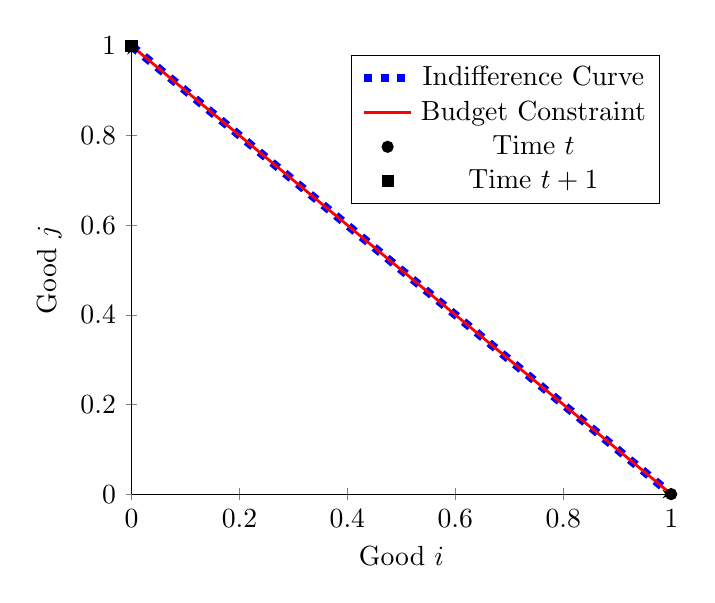
\begin{tikzpicture}
    \begin{axis}[
    axis lines = left,
    xlabel = Good $i$,
    ylabel = Good $j$
]
\addplot [
    domain=0:1, 
    samples=2, 
    color=blue,
    line width=3pt,
    dashed
]
{1-x};
\addlegendentry{Indifference Curve}
  \addplot [
    domain=0:1, 
    samples=2, 
    color=red,
    line width=1pt,
]
{1-x};
\addlegendentry{Budget Constraint}
\addplot [only marks] table {
1 0
};
\addlegendentry{Time $t$}
\addplot [only marks, mark=square*] table {
0 1
};
\addlegendentry{Time $t+1$}
    \end{axis}
\end{tikzpicture}
\end{center}
\noindent
Note the straight line represent both the indifference curves \emph{and} budget constraints at time $t$ both times. Under these conditions, any choice along the budget constraint is rational. 

The following table and Venn Diagram summarizes the requirements for each of the axioms:

\renewcommand{\arraystretch}{1.5}
\begin{center}
\begin{tabular}{ c|c|c } 
Axiom & If $\ldots$ & Then $\ldots$ \\\hline
WARP&$X_i \mathbf{R_D} X_j$&$\neg(X_j \mathbf{R_D} X_i)$ \\
SARP&$X_i \mathbf{R} X_j$&$\neg(X_j \mathbf{R} X_i)$ \\
WGARP&$X_i  \mathbf{R_D} X_j$&$\neg(X_j \mathbf{R_{SD}} X_i)$ \\
GARP&$X_i \mathbf{R} X_j$&$\neg(X_j  \mathbf{R_{SD}} X_i)$
\end{tabular}
\end{center}
\renewcommand{\arraystretch}{1}

\begin{center}
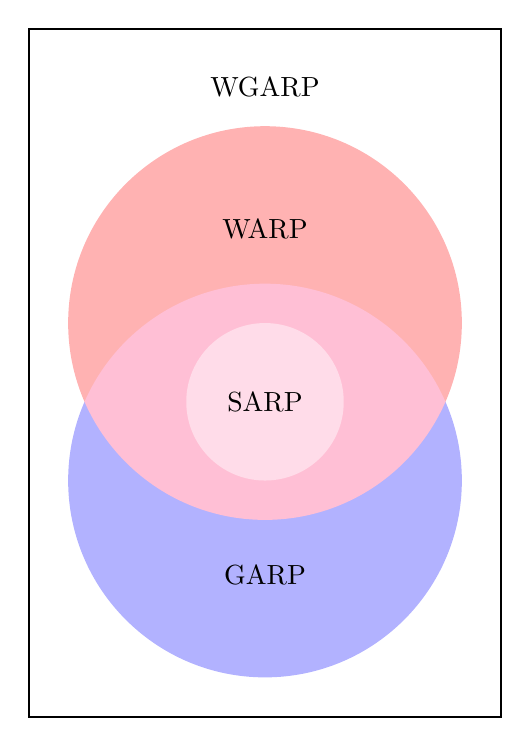
\begin{tikzpicture}
  \begin{scope}[blend group=soft light]
      \fill[red!30!white]   (90:2) circle (2.5);
    \fill[white!30!white] (90:1) circle (1);
    \fill[blue!30!white] (90:0) circle(2.5);
     \end{scope}
  \node at ( 90:3.2)    {WARP};
  \node at (90:1) {SARP};
  \node at (90:-1.2) {GARP};
  \node at (90:5) {WGARP};
    \draw[thick] ([shift={(-.5,-.5)}]current bounding box.south west) rectangle ([shift={(.5,.5)}]current bounding box.north east);
\end{tikzpicture}
\end{center}

\section*{Revealed Preferences as Directed Graphs}

This section will rigorously outline a graph theoretical approach to analyzing revealed preferences and introduce algorithms to test for each of the axioms. First, define two directed graphs, $G_d$ and $G_s$, that represent non-strict and strict relations between bundles, respectively. These conditions will yield:
$$G_d=\{\mathcal{X},E_d\}\textrm{ such that }E_d=\{(X_i,X_j)\ |\ X_i R_D X_j,\ i.e.\ P_iX_i\geq P_iX_j,\ i\not=j\}$$
$$G_s=\{\mathcal{X},E_s\}\textrm{ such that }E_s=\{(X_i,X_j)\ |\ X_i R_{SD} X_j,\ i.e.\ P_iX_i> P_iX_j,\ i\not=j\}$$
It is best to represent each graph with an adjacency matrix, where the $(i,j)^{th}$ element of the adjacency matrix is 1 if there's an edge from $X_i$ to $X_j$, 0 otherwise. The following paragraphs will discuss the construction of the adjacency matrices for $G_d$ and $G_s$, which will be denoted as $A_d$ and $A_s$, respectively.

Suppose an individual has choice data $\mathcal{X}=\{X_1,\ldots,X_k\}$ and $\mathcal{P}=\{P_1,\ldots,P_k\}$. One can then create the following $(k\times k)$ matrix from $\mathcal{X}$ and $\mathcal{P}$ (referred to as the expenditure matrix):
\[
Exp = 
 \begin{pmatrix}
  P_1X_1 & P_2X_1 & \cdots & P_kX_1 \\
  P_1X_2 & P_2X_2 & \cdots & P_kX_2 \\
  \vdots  & \vdots  & \ddots & \vdots  \\
  P_1X_k & P_2X_k & \cdots & P_kX_k
 \end{pmatrix}
\]
Note that the $(i,j)^{th}$ entry of this matrix represents the cost of bundle $i$ at the price of time $j$ (i.e. $P_jX_i$). Then consider the following:
\[
Exp_{diag} = 
 \begin{pmatrix}
  P_1X_1 & P_2X_2 & \cdots & P_kX_k \\
  P_1X_1 & P_2X_2 & \cdots & P_kX_k \\
  \vdots  & \vdots  & \ddots & \vdots  \\
  P_1X_1 & P_2X_2 & \cdots & P_kX_k
 \end{pmatrix}
\]
In $Exp_{diag}$, every element in column $j$ is same for all $j$ and represents the actual cost of bundle $j$ at the price vector it was bought at (price vector of time $j$). Then consider the following:
\[
\alpha = Exp-Exp_{diag} =
 \begin{pmatrix}
  0 & P_2X_1-P_2X_2 & \cdots & P_kX_1-P_kX_k \\
  P_1X_2-P_1X_1 & 0 & \cdots & P_kX_2-P_kX_k \\
  \vdots  & \vdots  & \ddots & \vdots  \\
  P_1X_k-P_1X_1 & P_2X_k-P_2X_2 & \cdots & 0
 \end{pmatrix}
\]
Define a function $f:\mathbb{R}\to\{0,1\}$ such that:
\[ 
f(x)=
    \begin{cases} 
      1 & x\leq0 \\
      0 & x>0
   \end{cases}
\]
Applying $f$ to all elements of $\alpha$ except its diagonals and take its transpose, one will obtain the adjacency matrix ($A_d$) for $G_d$:
\[
A_d =
 \begin{pmatrix}
  0 & f(\alpha_{1,2}) & \cdots & f(\alpha_{1,k}) \\
  f(\alpha_{2,1}) & 0 & \cdots & f(\alpha_{2,k}) \\
  \vdots  & \vdots  & \ddots & \vdots  \\
  f(\alpha_{k,1}) & f(\alpha_{k,2}) & \cdots & 0
 \end{pmatrix} ^T
\]
One can see that $A_d$ is in fact the adjacency matrix by considering the following:
\begin{itemize}
    \item $f(\alpha_{i,j})=1$ if and only if $\alpha_{i,j}\leq0$
    \item If $\alpha_{i,j}\leq0$, then $P_jX_i-P_jX_j\leq0$ and hence $P_jX_i\leq P_jX_j$
    \item Hence, by definition, $X_j R_D X_i$
    \item Thus $f(\alpha_{i,j})=1$ exactly when $X_j R_D X_i$
    \item However, a value of $1$ in $(i,j)$ position would indicate that a directed edge from vertex $i$ to vertex $j$, but since the edges need to indicate directly revealed preferences, one would want a value of $1$ at the $(j,i)$ positions. Hence, taking the transpose would result in $A_{d_{j,i}}=f(\alpha_{i,j})=1$ if and only if $X_j R_D X_i$, which is the desired adjacency matrix.
\end{itemize}
To construct $A_s$, consider the function $g:\mathbb{R}\to\{0,1\}$ such that:
\[ 
g(x)=
    \begin{cases} 
      1 & x<0 \\
      0 & x\geq0
   \end{cases}
\]
Similarly, applying $g$ to all elements of $\alpha$ except its diagonals and take its transpose would generate the adjacency matrix ($A_s$) for $G_s$:
\[
A_s =
 \begin{pmatrix}
  0 & g(\alpha_{1,2}) & \cdots & g(\alpha_{1,k}) \\
  g(\alpha_{2,1}) & 0 & \cdots & g(\alpha_{2,k}) \\
  \vdots  & \vdots  & \ddots & \vdots  \\
  g(\alpha_{k,1}) & g(\alpha_{k,2}) & \cdots & 0
 \end{pmatrix} ^T
\]
The intuition behind $A_s$ is similar to that of $A_d$ except the conditions of $g$ are set such that the relation between $X_i$ and $X_j$ need to be strict in order for $(i,j)$ to be 1.

Using the graph theoretical approach, one can reframe the relations on Definition \ref{defn:relations_1} as follows:
\begin{definition}\label{defn:relations_2} \leavevmode
\begin{enumerate}
  \circleditem For $X_i,X_j\in\mathcal{X}$, we say $X_i$ is \textbf{directly revealed preferred} to $X_j$ if there exists an edge from $X_i$ to $X_j$ on $G_d$, i.e. $(X_i,X_j)\in E_d$.
  \circleditem For $X_i,X_j\in\mathcal{X}$, we say $X_i$ is \textbf{strictly directly revealed preferred} to $X_j$ if there exists an edge from $X_i$ to $X_j$ on $G_s$, i.e. $(X_i,X_j)\in E_s$.
  \circleditem For $X_i,X_j\in\mathcal{X}$, we say $X_i$ is \textbf{revealed preferred} to $X_j$ if there's a walk (of any length) from $X_i$ to $X_j$ on $G_d$.
\end{enumerate}
\end{definition}
\noindent
Similarly, the axioms from Definition \ref{defn:axioms_1} is reframed as follows:

\begin{definition}\label{axioms_2} \leavevmode
\begin{enumerate}
  \circleditem A set of choice data satisfies the \textbf{Weak Axiom of Revealed Preferences (WARP)} if $\forall i,j\in\{1,\dots,k\}$ where $i\not=j$, if $(X_i,X_j)\in E_d$, then $(X_j, X_i)\not\in E_d$.
  \circleditem A set of choice data satisfies the \textbf{Strong Axiom of Revealed Preferences (SARP)} if $\forall X_i \in \mathcal{X}$, there exists no directed walk from $X_i$ back to itself.
  \circleditem A set of choice data satisfies the \textbf{Generalized Axiom of Revealed Preferences (GARP)} if $\forall i,j\in\{1,\dots,k\}$, if there exists a directed walk from $X_i$ to $X_j$ in $G_d$, then $(X_j,X_i)\not\in E_s$.
  \circleditem A set of choice data satisfies the \textbf{Weak Generalized Axiom of Revealed Preferences (WGARP)} if $\forall i,j\in\{1,\dots,k\}$ where $i\not=j$, if $(X_i,X_j)\in E_d$, then $(X_j, X_i)\not\in E_s$.
\end{enumerate}
\end{definition}
Suppose there exists a set of choice data for an individual given by $\{\mathcal{X},\mathcal{P}\}$ where $|\mathcal{X}|=|\mathcal{P}|=k\in\mathbb{N}$. Let $A_d$ and $A_s$ be the adjacency matrices of $G_d$ and $G_s$ constructed from the data set, respectively. To test for each of the axioms, the paper proposes the following theorems.
\begin{restatable}{thm}{WARP}
\label{thm:WARP}
A set of choice data, $\{\mathcal{X},\mathcal{P}\}$, satisfies WARP exactly when, $\forall i\in\{1,\ldots,k\}$, $(A_d)^2_{i,i}=0$.
\end{restatable}

WARP requirements are defined such that if $(\mathcal{X},\mathcal{P})$ passes WARP, then: $\forall i,j\in\{1,\dots,k\}$ where $i\not=j$, if $(X_i,X_j)\in E_d$, then $(X_j, X_i)\not\in E_d$. Note that this is true exactly when there \textit{isn't} a directed walk of length 2 from any vertex $i$ back to itself (vertex $i$). Hence we say $(\mathcal{X},\mathcal{P})$ passes WARP if and only if the main diagonal of matrix $(A_d)^2$ is a vector of 0, which is exactly the statement of Theorem \ref{thm:WARP}.

\begin{restatable}{thm}{SARP}
\label{thm:SARP}
A set of choice data, $\{\mathcal{X},\mathcal{P}\}$, satisfies SARP exactly when, $\forall i\in\{1,\ldots,k\}$, $(\sum_{n=2}^kA_d^n)_{i,i}=0$.
\end{restatable}
Let $B_d=(\sum_{n=2}^kA_d^n)$. Then $(B_d)_{i,j}>0$ if and only if there is a directed walk of at least length 2 from $X_i$ to $X_j$, as the cardinality of the vertex set is $k$ and adding above that index would simply be extra computation. Hence, $(B_d)$'s main diagonal is 0 if and only if no vertices has a directed walk back to itself, which is exactly the statement of Theorem \ref{thm:SARP}.

\begin{restatable}{thm}{WGARP}
\label{thm:WGARP}
A data set $(\mathcal{X}, \mathcal{P})$ passes WGARP if and only if, $\forall i\in\{1,\ldots,k\}$, $(A_d \times A_s)_{i,i}=0$ (i.e. the main diagonal of $A_d \times A_s$ is a vector of 0).
\end{restatable}

\begin{restatable}{thm}{GARP}
\label{thm:GARP}
A data set $(\mathcal{X},\mathcal{P})$ passes GARP if and only if, $\forall i\in\{1,\ldots,k\}$, $\big((\sum_{i=1}^{k-1}A_{d}^{i})\times A_s\big)_{i,i}=0$ (i.e. the main diagonal of $(\sum_{i=1}^{k-1}A_{d}^{i})\times A_s$ is a vector of 0).
\end{restatable}

The proofs of Theorem \ref{thm:WGARP} and Theorem \ref{thm:GARP} are in the Appendix. The basic idea behind these two algorithms are similar to that of Theorem \ref{thm:WARP} and Theorem \ref{thm:SARP}, except they are adjust to include the idea of strict revealed preferences that are a part of the axioms. This section will conclude with a few examples that exhibit the functionalities of the graph theoretical approach.

Consider the following data for a single consumer in 3 different time periods:
\begin{center}
\begin{tabular}{ cccccc } 
Choice Number & $p_{1}$ & $p_{2}$ & $x_{1}$ & $x_{2}$ \\
1&1&2&1&2 \\
2&2&1&2&1 \\
3&1&1&2&2
\end{tabular}
\end{center}
Then, $\forall n\in\{1,2,3\}$, calculate $P_{n}X_{n}$ and $\forall i,j\in\{1,2,3\}$ such that $i\not=j$, calculate $P_{j}X_{i}$. This will result in the following expenditure matrix:
\[
Exp = \begin{pmatrix}
5&4&3 \\
4&5&3 \\
6&6&4
\end{pmatrix}
\]
Using $Exp_{diag}$ as defined previously, calculate:
\[\alpha=Exp-Exp_{diag}=\begin{pmatrix}
0 &-1 &-1\\
-1&0&-1\\
1&1&0\\
\end{pmatrix}
\]
Applying $f$ to all non-diagonal elements of $\alpha$ and taking the inverse would result in the adjacency matrix, as follows:
\[
A_d=\begin{pmatrix}
0 & 1 & 0\\
1 & 0 &0 \\
1 & 1 & 0
\end{pmatrix}
\]
Since all the inequalities are strict in this case, we have $A_s=A_d$ and hence $G_s=G_d$. Consider the following graph, representing both $G_d$ and $G_s$:
\begin{center}
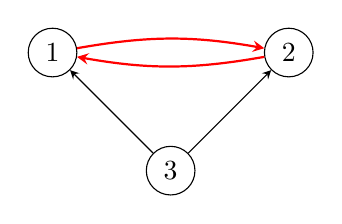
\begin{tikzpicture}[scale = 1.5]
\tikzset{
    vertex/.style={circle,draw,minimum size=1.5em},
    edge/.style={->,> = latex'}
}
  % vertices
\node[vertex] (1) at  (-1,0) {$1$};
\node[vertex] (2) at (1,0) {$2$};
\node[vertex] (3) at (0,-1) {$3$};
% edges
\path[->,>=stealth]
(1) edge[bend left=10,red,thick] (2)
(2) edge[bend left=10,red,thick] (1)
(3) edge (2)
(3) edge (1)
;
\end{tikzpicture}
\end{center}
Upon first glance, one can see that the revealed preferences between $X_1$ and $X_2$ indicates violations of all axioms. Since $G_d=G_s$, the individual's data set show that $(X_1,X_2)\in E_d = E_s$ and $(X_2,X_1)\in E_d=E_s$. This ``conflict'' is represented in the graph with the red arrows, creating a walk of 2 edges from $X_1$ back to itself (similarly with $X_2$). Theorem \ref{thm:WARP} states that, if the data set were to in fact fail WARP, there will be at least one non-zero element in the main diagonal of $(A_d)^2$. Using $A_d$ exhibited by the individual, one can see Theorem \ref{thm:WARP} holds:
\[
(A_d)^2=\begin{pmatrix}
0 & 1 & 0\\
1 & 0 &0 \\
1 & 1 & 0
\end{pmatrix}^2 = \begin{pmatrix}
1&0&0\\
0&1&0\\
1&1&0
\end{pmatrix}\]
Additionally, since $A_d=A_s$, $A_d\times A_s=A_d\times A_d=(A_d)^2$. Thus, the behavior exhibited by this individual fails WGARP as well.
\section*{Appendix}
\WGARP*

\begin{proof}
Recall that: If $(\mathcal{X},\mathcal{P})$ passes WGARP, then: $\forall i,j\in\{1,\dots,k\}$ where $i\not=j$, if $(X_i,X_j)\in E_d$, then $(X_j, X_i)\not\in E_s$. Which, when put in context of adjacency matrices, means that $\forall i,j\in\{1,\dots,k\}$ where $i\not=j$, if $(i,j)^{th}$ position of $A_d$ ($A_{d_{i,j}}$) is equal to one, then the $(j,i)^{th}$ position of $A_s$ ($A_{s_{i,j}}$) cannot be equal to 1. We then consider $A_d\times A_s$ and its main diagonal. 


$\forall i\in\{1,\ldots,k\}$, let $\delta_i$ be the vector of the $i^{th}$ row of $A_d$ and $\xi_i$ be the vector of the $i^{th}$ column of $A_s$. Then we have $(A_d\times A_s)_{i,i}=\delta_i\cdot\xi_i$. Note that $\delta_{i_i}=0$ and $\xi_{i_i}=0$ since originally $A_d$ and $A_s$ have all 0's across their main diagonals.


We then know that, $\forall i\in\{1,\ldots,k\}$, $(A_d\times A_s)_{i,i}=0$ (i.e. the main diagonal of $A_d\times A_s$ is a zero vector) if and only if $\delta_i\cdot\xi_i=0$. Further, $\delta_i\cdot\xi_i=0$ if and only if $\forall j \in\{1,\ldots,k\}$ such that $i\not=j$, $\delta_{i_j}\cdot \xi_{i_j}=0$ (since we know that $\delta_{i_i}=\xi_{i_i}=0$, they won't contributed to the overall sum, which is what we want anyways by the WGARP rules). We then know that $\delta_{i_j}\cdot \xi_{i_j}=0$ if and only if $\delta_{i_j}=0$ or $\xi_{i_j}=0$. Further, ``$\delta_{i_j}=0$ or $\xi_{i_j}=0$'' if and only if $\neg (\delta_{i_j}=\xi_{i_j}=1)$ (since all terms in $A_d$ and $A_s$ are either one or zero). Note that $\delta_{i_j}=A_{d_{i,j}}$ and $\xi_{i_j}=A_{s_{j,i}}$ (since $\xi_i$ is the vector of the $i^{th}$ \textit{column} of $A_s$). Hence, $\neg (\delta_{i_j}=\xi_{i_j}=1)$ if and only if $\neg (A_{d_{i,j}}=A_{s_{j,i}}=1)$, which happens if $A_{d_{i,j}}=1$, then $A_{s_{j,i}}=0\not=1$. Note that this is the exact definition of passing WGARP. Summarizing this, we have:
\begin{flalign*}
\forall i\in\{1,\ldots,k\}, (A_d\times A_s)_{i,i}=0 &\iff \delta_i\cdot\xi_i=0 &\\
&\iff \forall j \in\{1,\ldots,k\}\textrm{, }i\not=j,\ \delta_{i_j}\cdot \xi_{i_j}=0 &\\
&\iff \delta_{i_j}=0\textrm{ or }\xi_{i_j}=0 &\\
&\iff \neg (\delta_{i_j}=\xi_{i_j}=1) &\\
&\iff \neg (A_{d_{i,j}}=A_{s_{j,i}}=1) &\\
&\iff (A_{d_{i,j}}=1 \implies A_{s_{j,i}}=0\not=1)
\end{flalign*}

Hence, $\forall i, j\in\{1,\ldots,k\}$ such that $i\not=j$, $(A_d\times A_s)_{i,i}=0 \iff (A_{d_{i,j}}=1 \implies A_{s_{j,i}}=0\not=1)$. Note the first statement simply means the main diagonal of $A_d\times A_s$ is the zero vector and the second statement is the condition for passing WGARP. We then have ``passing WGARP'' $\iff$ ``main diagonal of $A_d\times A_s$ is a zero vector''. Thus our claim is proven (since $A\iff B$ is the same as $B\iff A$).
\end{proof}

\GARP*

Before we begin the proof, consider the following lemma:

\begin{lemma}
\label{lma:LemmaA}
Let $X_1, X_2, Y$ be $(m\times m)$ matrices such that:

\begin{minipage}{.5\linewidth}
\[
X_1 =
 \begin{pmatrix}
  x_{1,1} & x_{1,2} & \cdots & x_{1,m} \\
  x_{2,1} & x_{2,2} & \cdots & x_{2,m} \\
  \vdots  & \vdots  & \ddots & \vdots  \\
  x_{m,1} & x_{m,2} & \cdots & x_{m,m}
 \end{pmatrix}
\]
\end{minipage}
\begin{minipage}{.5\linewidth}
\[
X_2 =
 \begin{pmatrix}
  0 & x_{1,2} & \cdots & x_{1,m} \\
  x_{2,1} & 0 & \cdots & x_{2,m} \\
  \vdots  & \vdots  & \ddots & \vdots  \\
  x_{m,1} & x_{m,2} & \cdots & 0
 \end{pmatrix}
\]
\end{minipage}
and 

\[
Y =
 \begin{pmatrix}
  0 & y_{1,2} & \cdots & y_{1,m} \\
  y_{2,1} & 0 & \cdots & y_{2,m} \\
  \vdots  & \vdots  & \ddots & \vdots  \\
  y_{m,1} & y_{m,2} & \cdots & 0
 \end{pmatrix}
\]

Then the main diagonals of $X_1\times Y$ and $X_2\times Y$ are the same (denoted $diag(X_1\times Y)=diag(X_2\times Y)$).
\end{lemma}

\begin{proof}
Fix an arbitrary $i\in\{1,\ldots,m\}$. Then let $Z_1=X_1\times Y$ and $Z_2=X_2\times Y$. We want to show that $Z_{1_{i,i}}=Z_{2_{i,i}}$. Note that $Z_{1_{i,i}}=x_{i,1}y_{1,i}+x_{i,2}y_{2,i}+\ldots+x_{i,i}y_{i,i}+\ldots+x_{i,m}y_{m,i}$ and that $Z_{2_{i,i}}=x_{i,1}y_{1,i}+x_{i,2}y_{2,i}+\ldots+0y_{i,i}+\ldots+x_{i,m}y_{m,i}$. The only difference between those are that for the first equation, we have $x_{i,i}y_{i,i}$ as the $i^{th}$ term and the second equation, we have $0y_{i,i}$ as the $i^{th}$ term. However, since $y_{i,i}=0$, we have that $x_{i,i}y_{i,i}=0y_{i,i}=0$ and thus $Z_{1_{i,i}}=Z_{2_{i,i}}$.
\end{proof}

Now, consider the following proof for Theorem \ref{thm:GARP}:
\begin{proof}
The proof of this will look very similar to the proof of WGARP, except that the elements in $\sum_{i=1}^{k-1}A_{d}^{i}$ will no longer be binary $(\{0,1\})$. However, they are all $\geq0$. Let $\beta_d=\sum_{i=1}^{k-1}A_{d}^{i}$, then $\beta_{d_{i,j}}$ would be the number of directed walks between vertex $i$ and vertex $j$ of any length up to $k-1$. Note that we chose to sum up to $k-1$ since anything past that, we would definitely have a cycle and summing past that point is redundant.


We want to make sure that if there's a directed walk from vertex $i$ to vertex $j$ in $G_d$, there isn't a directed edge between vertex $j$ and vertex $i$ in $G_s$. Formally, this is just our definition for GARP: If $(\mathcal{X},\mathcal{P})$ passes GARP, then: $\forall i,j\in\{1,\dots,k\}$, if there exists a directed walk from $X_i$ to $X_j$ in $G_d$, then $(X_j,X_i)\not\in E_s$. This is similar to WGARP in the sense that we're simply replacing the directed edge in the ``if'' statement to a directed walk. Note then that we have $\beta_d=\sum_{i=1}^{k-1}A_{d}^{i}$, which captures the existence of any directed walks between any two verices. Hence if $\beta_{d_{i,j}}>0$, there exists at least 1 directed walk between vertex $i$ and vertex $j$ on graph $G_d$. We can then use our proof for WGARP and \textit{Lemma A} to construct the rest of this proof.


In our proof of WGARP, we see that $\forall i, j\in\{1,\ldots,k\}$ such that $i\not=j$, $(A_d\times A_s)_{i,i}=0 \iff (A_{d_{i,j}}=1 \implies A_{s_{j,i}}=0\not=1)$. There are two changes we need to make to this statement to fit our GARP claim. 

First, we see that we're no longer working with $A_d$ but working with $\beta_d$, which represents directed walks instead of edges. $\beta_d$ is also no longer filled with binary elements $\in\{0,1\}$. We can tweak our statement to fit these conditions by stating: $\forall i, j\in\{1,\ldots,k\}$ such that $i\not=j$, $(\beta_d\times A_s)_{i,i}=0 \iff (\beta_{d_{i,j}}>0 \implies A_{s_{j,i}}=0)$. Now, $\beta_{d_{i,j}}>0$ simply means there exists at least one path from $i,j$ regardless of length, which is what we want.

Second, when we constructed our proof of WGARP, we noted that ``since we know that $\delta_{i_i}=\xi_{i_i}=0$ (i.e. $A_{d_{i,i}}=0$ and $A_{s_{i,i}}=0$), they won't contributed to the overall sum, which is what we want anyways by the WGARP rules''. However, this no longer holds as we could have $\beta_{d_{i,i}}\not=0$ for some $i$ if there's any directed cycles in $G_d$ (but we don't care about those in GARP, per the definition of the axiom). But we do still have $A_{s_{i,i}}=0$ for all $i$ and thus, by \textit{Lemma A}, we don't need to ``clear-out'' the diagonals of $\beta_d$ before multiplying. Hence, our statement above still holds. 

Thus, we have: $\forall i, j\in\{1,\ldots,k\}$ such that $i\not=j$, $(\beta_d\times A_s)_{i,i}=0 \iff (\beta_{d_{i,j}}>0 \implies A_{s_{j,i}}=0)$. The first statement simply means the main diagonal of $(\beta_d=\sum_{i=1}^{k-1}A_{d}^{i}\times A_s)$ is a zero vector and the second statement is the condition for passing GARP, hence our proof is complete (since $A\iff B$ is the same as $B\iff A$).
\end{proof}

\bibliographystyle{plainnat}
\bibliography{bibliography}

\end{document}
